\PassOptionsToPackage{unicode=true}{hyperref} % options for packages loaded elsewhere
\PassOptionsToPackage{hyphens}{url}
%
\documentclass[ignorenonframetext,]{beamer}
\usepackage{pgfpages}
\setbeamertemplate{caption}[numbered]
\setbeamertemplate{caption label separator}{: }
\setbeamercolor{caption name}{fg=normal text.fg}
\beamertemplatenavigationsymbolsempty
% Prevent slide breaks in the middle of a paragraph:
\widowpenalties 1 10000
\raggedbottom
\setbeamertemplate{part page}{
\centering
\begin{beamercolorbox}[sep=16pt,center]{part title}
  \usebeamerfont{part title}\insertpart\par
\end{beamercolorbox}
}
\setbeamertemplate{section page}{
\centering
\begin{beamercolorbox}[sep=12pt,center]{part title}
  \usebeamerfont{section title}\insertsection\par
\end{beamercolorbox}
}
\setbeamertemplate{subsection page}{
\centering
\begin{beamercolorbox}[sep=8pt,center]{part title}
  \usebeamerfont{subsection title}\insertsubsection\par
\end{beamercolorbox}
}
\AtBeginPart{
  \frame{\partpage}
}
\AtBeginSection{
  \ifbibliography
  \else
    \frame{\sectionpage}
  \fi
}
\AtBeginSubsection{
  \frame{\subsectionpage}
}
\usepackage{lmodern}
\usepackage{amssymb,amsmath}
\usepackage{ifxetex,ifluatex}
\usepackage{fixltx2e} % provides \textsubscript
\ifnum 0\ifxetex 1\fi\ifluatex 1\fi=0 % if pdftex
  \usepackage[T1]{fontenc}
  \usepackage[utf8]{inputenc}
  \usepackage{textcomp} % provides euro and other symbols
\else % if luatex or xelatex
  \usepackage{unicode-math}
  \defaultfontfeatures{Ligatures=TeX,Scale=MatchLowercase}
\fi
% use upquote if available, for straight quotes in verbatim environments
\IfFileExists{upquote.sty}{\usepackage{upquote}}{}
% use microtype if available
\IfFileExists{microtype.sty}{%
\usepackage[]{microtype}
\UseMicrotypeSet[protrusion]{basicmath} % disable protrusion for tt fonts
}{}
\IfFileExists{parskip.sty}{%
\usepackage{parskip}
}{% else
\setlength{\parindent}{0pt}
\setlength{\parskip}{6pt plus 2pt minus 1pt}
}
\usepackage{hyperref}
\hypersetup{
            pdftitle={Assessing incomplete sampling of disease transmission networks},
            pdfauthor={Derek Sonderegger, PhD - Northern Arizona University},
            pdfborder={0 0 0},
            breaklinks=true}
\urlstyle{same}  % don't use monospace font for urls
\newif\ifbibliography
\setlength{\emergencystretch}{3em}  % prevent overfull lines
\providecommand{\tightlist}{%
  \setlength{\itemsep}{0pt}\setlength{\parskip}{0pt}}
\setcounter{secnumdepth}{0}

% set default figure placement to htbp
\makeatletter
\def\fps@figure{htbp}
\makeatother


\title{Assessing incomplete sampling of disease transmission networks}
\providecommand{\subtitle}[1]{}
\subtitle{PMI Monthly Meeting}
\author{Derek Sonderegger, PhD - Northern Arizona University}
\date{May 8, 2019}

\begin{document}
\frame{\titlepage}

\begin{frame}{Collaboration with NAU's Pathogen and Microbiome
Institute}
\protect\hypertarget{collaboration-with-naus-pathogen-and-microbiome-institute}{}

\begin{center}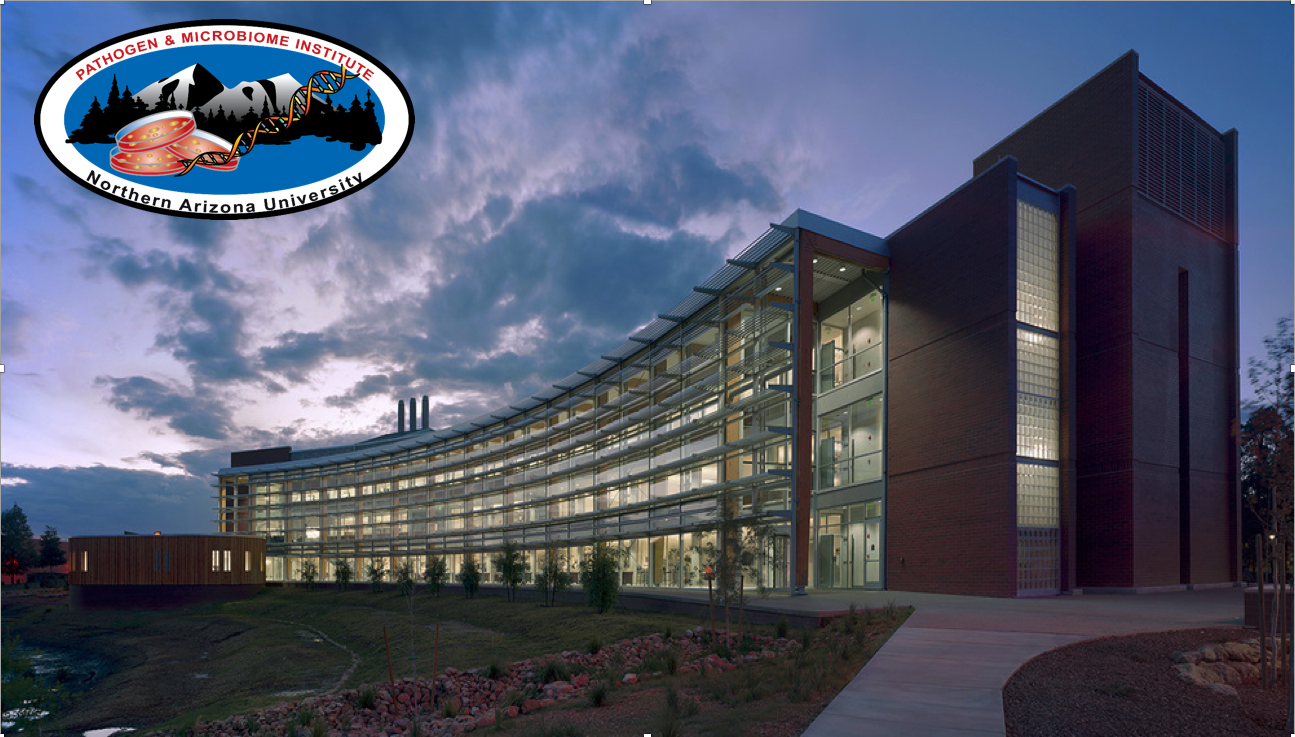
\includegraphics[width=600px]{Images/ARD&PMI} \end{center}

\end{frame}

\begin{frame}{Cluster Size Distributions}
\protect\hypertarget{cluster-size-distributions}{}

\begin{center}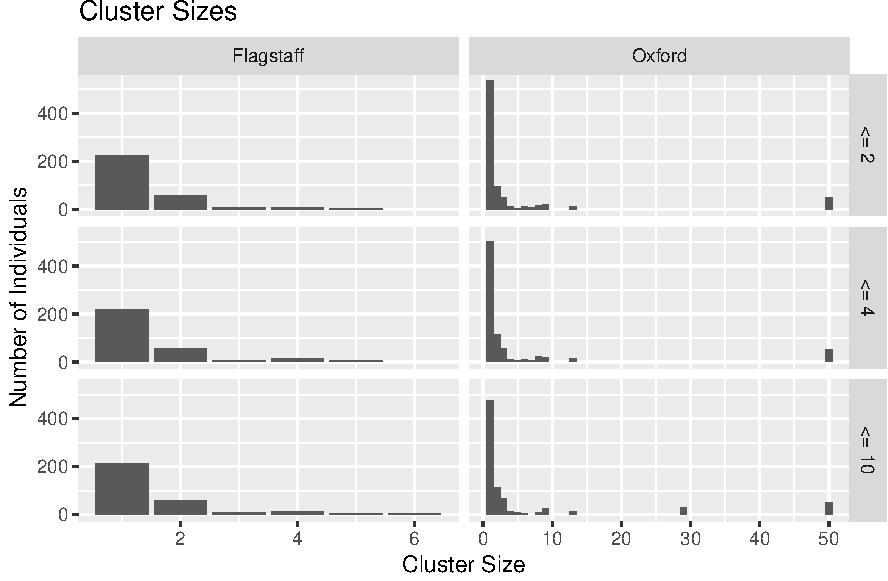
\includegraphics{Talk_PMI_files/figure-beamer/fig1-1} \end{center}

\end{frame}

\begin{frame}{Defining \(\gamma\) = HAI rate from full data}
\protect\hypertarget{defining-gamma-hai-rate-from-full-data}{}

\begin{itemize}
\tightlist
\item
  For each cluster, the first time a strain is observed it is considered
  environmentally acquired.
\item
  The second (or third, or fourth, ..) time a strain is observed, it is
  healthcare acquired.
\end{itemize}

\[ \gamma = \frac{N - ||\mathcal{I}||}{N} = 1 - \frac{||\mathcal{I}||}{N}\]
\[ N = \textrm{ Number of Patients }\]
\[\mathcal{I} = \textrm{ Set of strain identifiers }\]
\[||\mathcal{I}|| = \textrm{ Actual Number of Clusters/Strains }\]

\begin{itemize}
\tightlist
\item
  Knowing \(||\mathcal{I}||\) is the key to calculating HAI rate!
\end{itemize}

\end{frame}

\begin{frame}{Observed Number of Clusters/Strains under Simple Random
Sampling}
\protect\hypertarget{observed-number-of-clustersstrains-under-simple-random-sampling}{}

\begin{itemize}
\tightlist
\item
  Define the following
\end{itemize}

\[\alpha = \textrm{ proportion of the population sampled }\]
\[ n_i = \textrm{ actual size of the }i \textrm{th cluster}\]
\[ m_i = \textrm{ observed size of the }i \textrm{th cluster}\]

Notice that

\[1 \le m_i \le n_i\] and \[\sum n_i = N\] \[ \sum m_i = \alpha N\]

\[ \widehat{HAI}_{naive} = 1 - \frac{||I||}{n} \]
\[ n = \textrm{ sample size } \]

\end{frame}

\begin{frame}{Conditional Distribution}
\protect\hypertarget{conditional-distribution}{}

\[m_i | n_i \sim \textrm{ZTHyperGeometric}(n_i, \; N-n_i, \;\alpha N) \; \textrm{for}\; i \in I\]

\begin{itemize}
\tightlist
\item
  Zero Truncated HyperGeometric
\item
  Assume approximate independence between observed cluster sizes
\item
  Distribution requires working with hypergeometric terms
\end{itemize}

\[f(0|n_i) =  \frac{ {n_i \choose 0}{N-n_i \choose \alpha N} }{ {N \choose \alpha N}}\]

Notice that \(\alpha\) and \(f(0|n_i)\) are inversely related and we
could crudely approximate

\[f(0|n_i) \approx 1-\alpha\]

\end{frame}

\begin{frame}{Critical Expectation}
\protect\hypertarget{critical-expectation}{}

\[E[m_i] = E[ E(m_i|n_i)] = E[ (1-f(0|n_i))^{-1} \;\alpha \;n_i]\]

Utilizing this equation, can derive two different estimators.

\begin{enumerate}
\tightlist
\item
  The plug-in estimator that ignores the expectation, and approximates
  \(\left[ 1-f(0)\right]^{-1} \approx \alpha^{-1}\). This results in
  \(\widehat{n}_i = m_i\).
\item
  Ignoring the expectations, we could utilize the actual hypergeometric
  function for \(f(0|n_i)\) and solve the following equation for
  \(\widehat{n}_i\). This solution needs to be solved via numerical
  methods because the ``chooses'' in \(f(0|n_i)\).
\end{enumerate}

\end{frame}

\begin{frame}{Biased Estimator}
\protect\hypertarget{biased-estimator}{}

\begin{itemize}
\tightlist
\item
  Denoting
\end{itemize}

\[\widehat{n} = \sum\widehat{n}_i\]
\[ I = \textrm{ Set of observed strains }\]
\[ ||I|| = \textrm{ Observed Number of Clusters/Strains }\]
\[\widehat{\gamma}^* = \frac{1}{\widehat{n}}\sum_{i\in I} (\widehat{n}_i-1) = \frac{\widehat{n} - ||I||}{\widehat{n}} = 1-\frac{||I||}{\widehat{n}}\]

\end{frame}

\begin{frame}{Does the plug-in Estimator Work?}
\protect\hypertarget{does-the-plug-in-estimator-work}{}

\begin{center}\includegraphics{Talk_PMI_files/figure-beamer/unnamed-chunk-3-1} \end{center}

\end{frame}

\begin{frame}{Why doesn't this work?}
\protect\hypertarget{why-doesnt-this-work}{}

\begin{center}\includegraphics{Talk_PMI_files/figure-beamer/unnamed-chunk-4-1} \end{center}

\end{frame}

\begin{frame}{Bias Correction Procedure}
\protect\hypertarget{bias-correction-procedure}{}

\begin{enumerate}
\tightlist
\item
  Calculate the sample HAI rate.
\item
  Repeatedly subsample the sample at the designated \(\alpha\) fraction.
\item
  For each subsample, calculate the subsample's HAI rate
\item
  Look at the average discrepancy and use that to adjust the sample HAI
  rate estimate.
\item
  The adjustments are made on the logit scale to force the resulting
  rate to remain in the \([0,1]\) interval.
\end{enumerate}

\end{frame}

\begin{frame}{Bias Correction Procedure - Math!}
\protect\hypertarget{bias-correction-procedure---math}{}

By repeatedly sub-sampling at \(\alpha\) rate \(J\) times and
calculating \(\widehat{\gamma}^*_j\) for the \(j\)th sub-sample,

\[\bar{\delta} = \frac{1}{J}\sum\left[ \textrm{logit}(\widehat\gamma^*) - \textrm{logit}(\widehat\gamma^*_j) \right]\]

\[\widehat{\gamma} = \textrm{ilogit}\left( \textrm{logit}( \widehat{\gamma}^* ) + \bar\delta \right)\]

We performed the bias correction step on the logit scale to ensure the
resulting estimator is in \([0,1]\).

\end{frame}

\begin{frame}{Get approximate Confidence Intervals too!}
\protect\hypertarget{get-approximate-confidence-intervals-too}{}

\begin{itemize}
\tightlist
\item
  Standard deviation of the \(\textrm{logit}(\widehat\gamma^*_j)\)
  values gives a estimated standard error of
  \(\textrm{logit}(\widehat{\gamma})\) value.
\item
  An approximate \(95%\) confidence interval for \(\gamma\) we use is to
  add/subtract
\end{itemize}

\[\textrm{ilogit} \left[ \textrm{logit}(\widehat\gamma) \pm Z_{0.975}*SE(\textrm{logit}(\widehat\gamma))\right]\]

\end{frame}

\hypertarget{results}{%
\section{Results}\label{results}}

\begin{frame}{Plugin Results - Clinical Data}
\protect\hypertarget{plugin-results---clinical-data}{}

\begin{center}\includegraphics{Talk_PMI_files/figure-beamer/unnamed-chunk-5-1} \end{center}

\end{frame}

\begin{frame}{Hypergeometric Results - Clinical Data}
\protect\hypertarget{hypergeometric-results---clinical-data}{}

\begin{center}\includegraphics{Talk_PMI_files/figure-beamer/unnamed-chunk-6-1} \end{center}

\end{frame}

\begin{frame}{Results - Simulated Populations}
\protect\hypertarget{results---simulated-populations}{}

The Oxfordshire data could be reasonably modeled using a mixture of two
distributions to separate the small clusters sizes from the large. We
chose to model the small clusters sizes using a truncated Poisson
distribution with the zero truncated out. The large cluster sizes were
modeled from a logNormal distribution.

\[n_i \sim \begin{cases}
 \textrm{TPoisson}(\lambda)       & \textrm{ with probability } 1 - \rho \\
 \textrm{logNormal}(\mu, \sigma)  &\textrm{ with probability } \rho 
\end{cases}\]

for \(i\) in \(\mathcal{I}\).

\end{frame}

\begin{frame}{Simulated Data Populations}
\protect\hypertarget{simulated-data-populations}{}

\begin{center}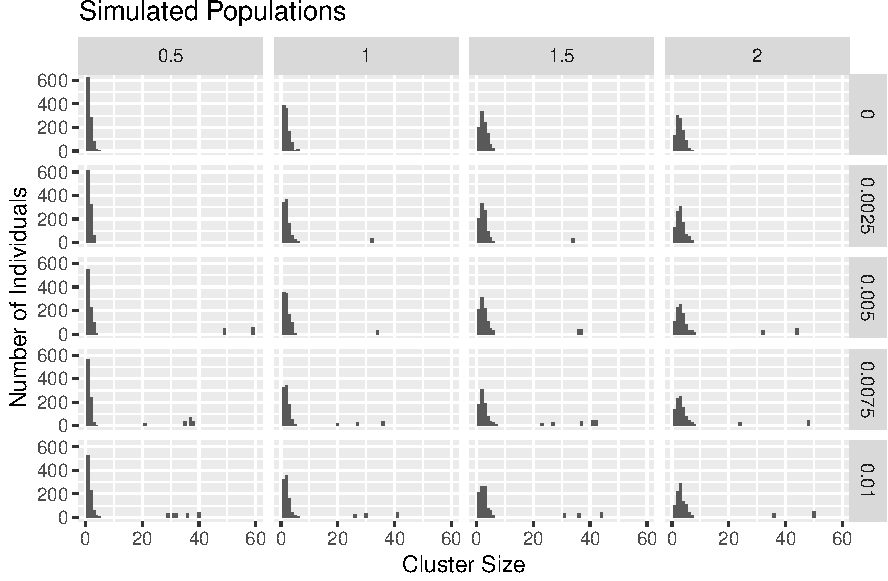
\includegraphics{Talk_PMI_files/figure-beamer/fig2-1} \end{center}

\end{frame}

\begin{frame}{Simulated Data Populations: Results}
\protect\hypertarget{simulated-data-populations-results}{}

\begin{center}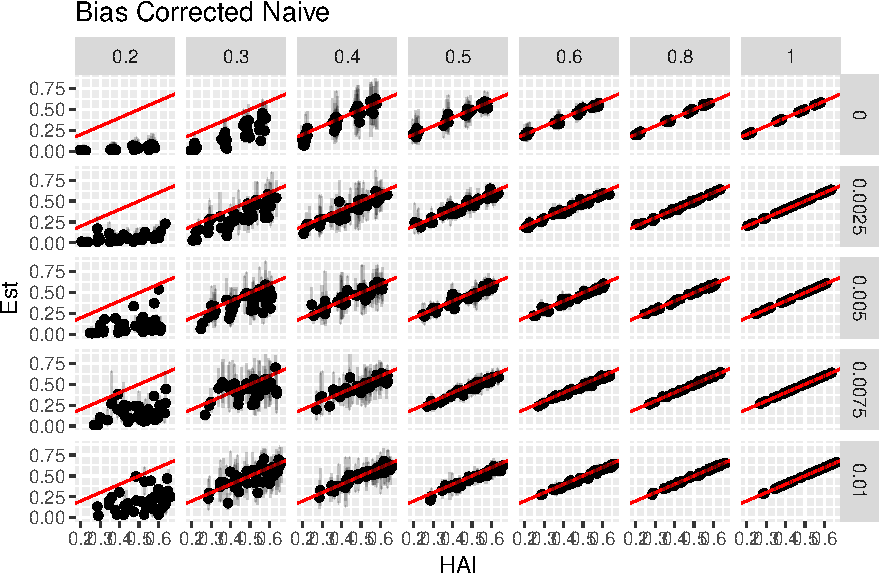
\includegraphics{Talk_PMI_files/figure-beamer/Graph_of_Generated_Populations2a-1} \end{center}

\end{frame}

\begin{frame}{Simulated Data Populations: Results}
\protect\hypertarget{simulated-data-populations-results-1}{}

\begin{center}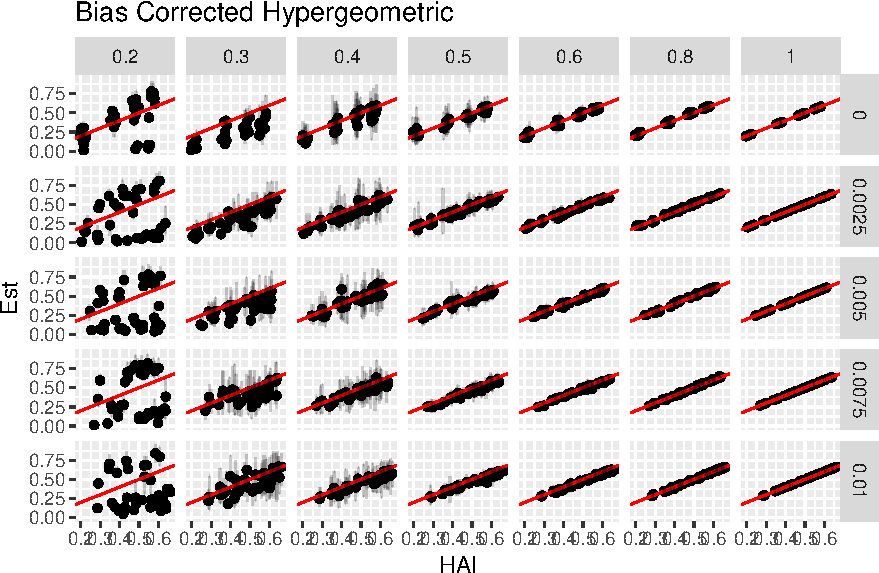
\includegraphics{Talk_PMI_files/figure-beamer/Graph_of_Generated_Populations2b-1} \end{center}

\end{frame}

\end{document}
